\chapter{Methodology}  \label{ch:methodology}

\begin{table}[h]
\centering
 \begin{tabular}{l l} 
 \hline
 SYMBOL & DESCRIPTION \\ 
 \hline
 $K$ & Number of Topics \\  
 $V$ & Number of words in the vocabulary \\
 $M$ & Number of documents \\
 $N$ & Number of words in the document \\
 $N_{d=1..M}$ & Number of words in document d\\
 $\alpha$ & Collection of all $\alpha$ \\
 $\alpha_{k=1...K}$ & Hyperparameter for dirichlet prior distribution of topic $k$ \\
 $\beta$ & collection of all $\beta$ \\
 $\beta_{w=1...V}$ & Hyperparameter for dirichlet prior distribution of a word $w$ in a topic \\
 $\varphi_{k=1...K}$ & Distribution of words in topic $k$ \\
 $\varphi_{k=1...K, w=1...V}$ & Probability of  word $w$ in topic $k$  \\
 $\theta{d=1...M}$ & Distribution of topics in document $d$  \\
 $\theta{d=1...M, k=1...K}$ & Probability of  topic $k$ in document $d$ \\
 $z_{d=1...M, w=1...N_d}$ & Assigned topic of word $w$ in document $d$\\
 $Z$ & Topic of all words in documents \\
 $w_{d=1...M, w=...N_d}$ & Assigned word w in document d \\ 
 $W$ & Words in all documents \\ 

 

 
 \hline
 \end{tabular}
\caption{Complete notation of LDA}
\label{tab:table1}
\end{table}

\section{Topic Modelling}
Topic models are algorithms used to find themes in mostly large unstructured collections of documents \cite{Blei2010ProbabilisticModels}. Where humans have a hard time to find a structure, topic modelling uses statistical methods for analysing words for topic discovery. This makes it possible to compare topics with each other, find similar documents without necessarily having any prior knowledge of your collection. 


\section{Latent dirichlet allocation}
In natural language processing \textit{Latent dirichlet allocation} (LDA) is an unsupervised machine learning technique introduced in 2003 for Topic modelling \cite{Blei2003LatentAllocation}. The formal notation for LDA can be seen in table \ref{tab:table1}.

LDA makes use of a generative probabilistic model of a collection of documents \textbf{M} (corpus) to discover latent topics, Fig \ref{fig:LDA} represents the plate notation of LDA. For a more understandable model take Fig \ref{fig:LDA_example}. This model assumes that each document \textbf{N} in the corpus contains a mixture of latent topics. These topics are a mixture of words \textbf{W} assigned to a topic from a fixed vocabulary \textbf{V}. \textbf{Z} notates the assignment of specific words to topics. The distribution of words $\theta$ for each topic is dependent on the sensitivity of $\alpha$. A low $\alpha$ means that the topic contains a distinct (sparse) representation of words and a high $\alpha$ means that topics have more generative words. The probability distribution of topics in documents $\varphi$ are depended on the sensitivity of $\beta$. A low $\beta$ means that documents contain distinct topics and a high $\beta$ is a mixture of multiple topics in a document. The number of topics \textbf{K} are predefined in LDA. 

\begin{figure}
    \centering
    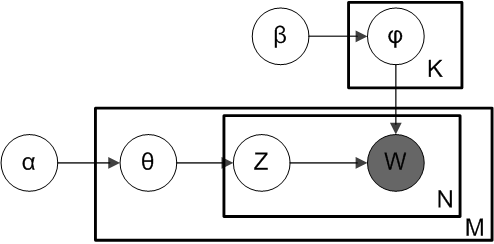
\includegraphics[width=10cm, height=5cm]{methodology/Smoothed_LDA.png}
    \caption{The smoothed LDA plate notation}
    \label{fig:LDA}
\end{figure}

The LDA algorithm is defined in 3 steps and shown in Fig \ref{fig:LDA_example}:
\begin{enumerate}
    \item For each document, pick a topic from its assigned distribution over topics.
    \item Sample a word from the distribution over the words associated with the chosen topic. 
    \item  The process is repeated for all the words in the document.
\end{enumerate}

In the original LDA model, assignments of words get updated every iteration through the corpus M. Restarting the process again until the LDA model converges and the topic and assignment are stale. The eventual quality of the model depends on the assumed hyperparameters $\alpha$ and $\beta$ and dirichlet parameters $\theta$ and $\varphi$. 

\begin{figure}
    \centering
    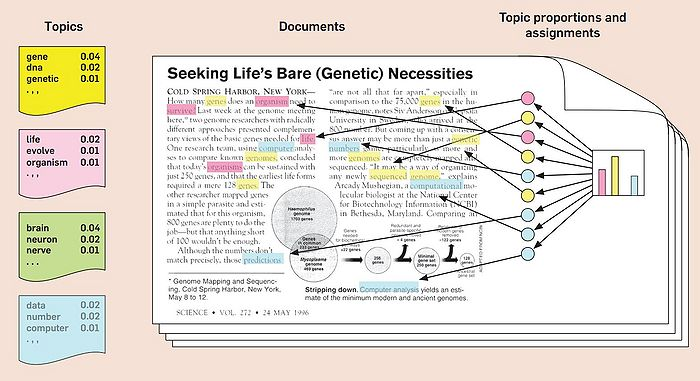
\includegraphics[scale=0.6]{methodology/700px-Illustrating_LDA.jpg}
    \caption{LDA applied to a document}
    \label{fig:LDA_example}
\end{figure}

\subsection{$\alpha$ and $\beta$ hyperparameters} 
Hyperparameters are defined as parameters that assume a prior distribution before any evidence or information is taken into account. This distinguishes $\alpha$ and $\beta$ from the remaining parameters. $\alpha$ is the parameter of the Dirichlet prior on the per-document topic distributions. $\beta$ is the parameter of the Dirichlet prior on the per-topic word distribution. The Dirichlet is defined as the distribution over a distribution.

\subsection{$\theta$, $\varphi$ parameters}
The parameters $\theta, \varphi$ are depend on the prior distributions $\alpha$ and $\beta$. $\theta$ is the document-topic distribution assumption. Because $\alpha$ is a prior distribution, $\theta$ assumes a distribution based on the previous assigned distribution. The same goes for $\varphi$. $\varphi$ in this case is dependent on the $\beta$. 

\section{Online Latent dirichlet allocation}
The online variant of LDA was introduced  by Hoffman et al. in 2010.\cite{Hoffman2010OnlineAllocation} This new variation dealt with the problem earlier LDA models struggled with. The problem that LDA had was the computing of huge collections of documents. The online lDA can be used for massive and streaming documents without losing performance compared to the original LDA model, because it analyses the documents in batches instead of single observations with stochastic (random) optimisation.\cite{Beaver2012StochasticInference} 

